
\section{Running on the FPGA}
This section talks about how to generate required files and steps to run the demo. \\
Note: 1) The text mark with \colorbox{blue!30}{\hspace{0.5cm}} means the command typed in terminal.\\
2) The text marked in \textcolor{green!100}{green} are the files that require manually modify.

\subsection{Process Overflow}
\begin{figure}[H]
	\includegraphics[scale=0.50]{fig/r2u2_fpga_flow.pdf}
	\caption{Deploying steps of R2U2 into an FPGA.}
	\label{fig:fpga_flow}
\end{figure}

\subsection{Introduction to Configuration File}
To generate the binary configuration file for the FPGA, user need to provide the following dependent files:
\begin{enumerate}
	\item \textbf{atomic checker (VHD file)}:
	All the sensor signals should be processed into atomic propositions in R2U2 by defining the atomic conversion functions. These functions will be conducted in hardware. User need to specify how many atomic checkers are required in hardware and the sensor input into each atomic checker. This procedure results in two VHDL files: \blue{at\_checkers.vhd} and \blue{log\_input\_pkg.vhd}. We have tools to support building the VHDL file, namely \green{inputs.py}, \blue{transformer.py} and \blue{util.py}. User only need to modify \green{inputs.py}. For details of \green{inputs.py}, refer to \ref{inputs.py}.

	\item \textbf{assert conversion configuration file}:
	Apart from specifying the atomic checker for the hardware, users also need to use the software to configure the atomic conversion function during R2U2 runtime. Basically, the configuration tells what number you want the sensor signal to compare with, or do you want to do the addtion/minus of two sensor signals first before the comparasion. The rules is written in the file \green{*.ast}. For the syntax of the rules, refer to \ref{input.ast}. Script \blue{assert\_convert.py} will convert the rules into binary format that the hardware can decode.
	\item \textbf{MLTL related file}:
	
	\item \textbf{sensor trace file}:
	User manually type the input in binary format as the sensor signal at each time stamp.
\end{enumerate}
User should modify the config.py file first before running any scripts. In the config.py file, user need to specify the following parameters:

\subsubsection{Run Mode}
We can specify the running mode in config.py file. The monitor has two running mode:
\begin{enumerate}
	\item \textbf{self\_sensing}:
	Read sensor signal on chip under the specified sample rate. This is what we show in the Oct.2018 demo video.
	\item \textbf{read\_log}:
	Read sensor signal from UART software. In this mode, the processed sensor in raw binary format will be send to FPGA through UART. The purpose of this mode is for debugging or regression test.
	\item \textbf{type\_input}:
	User manually type the input in binary format as the sensor signal at each time stamp.
\end{enumerate}

\subsection{Steps-Preparation}
Navigate to folder \blue{/tools/preprocessing/}
\begin{enumerate}
\item Modify general configuration file \\
	First, modify the configuration file \green{config.py}. This file sets the data width and running mode for R2U2.
\item Generate atomic checker associated file\\
	Go to folder \blue{/tools/preprocessing/at\_checker/}
	\begin{enumerate}
		\item Modify \green{inputs.py} (section \ref{inputs.py}) to specify the input data's format and name.
		\item Generate \textcolor{purple!30}{at\_checkers.vhd} and \textcolor{purple!30}{log\_input\_pkg.vhd}
		\begin{lstlisting}[language=Bash]
python transformer.py
		\end{lstlisting}
		\item Write atomic assertion configuration in \green{input.ast} (section \ref{input.ast}). 
		Go to folder \blue{/tools/preprocessing/}, use the following command to convert the assertion into binary configuration file named \textcolor{purple!30}{res.atc}.
		\begin{lstlisting}[language=Bash]
python assert_convert.py
		\end{lstlisting}
	\end{enumerate}
\item Generate binary instruction assembly code and its interval file (.ftasm, .ftm and .fti)
	\begin{enumerate}
		\item In folder \blue{tools/preprocessing/}
		\begin{lstlisting}[language=Bash]
(python 3) python ../Compiler/MLTL_main.py [MLTL]
		\end{lstlisting}
		This command generates assembly file \blue{tmp.ftasm} from MLTL.
		\begin{lstlisting}[language=Bash]
cat tmp.ftasm | ../AssemblyToBinary/ftas.py tmp
		\end{lstlisting}
			This command takes \blue{tmp.ftasm} as input and generates binary instruction file \blue{tmp.ftm} and \blue{tmp.fti}.
	\end{enumerate}
\item Generate UART byte data
		Run following command to generate \blue{*.uart} file. This file will be send through uart to FPGA.
		\begin{lstlisting}[language=Bash]
python gen_uart_data.py
		\end{lstlisting}		
\end{enumerate}

Note for VHDL code:
\begin{enumerate}
\item Current VHDL R2U2 uses the fixed SCQ size for each MLTL assmebly instruction. User can change the SCQ size by modifying parameter \tpurple{QUEUE\_SIZE} in \green{ft\_mu\_monitor\_pkg.vhd}.
\item To change the timestamp width, 1) revise parameter \tpurple{TIMESTAMP\_WIDTH} in \green{mu\_monitor\_pkg.vhd}. 2) Revise \tpurple{TIMESTAMP\_BYTE\_extend\_byte} in \green{config.py} (unit in byte). 
\end{enumerate}


\subsection{Steps-Execution}
Navigate to folder \blue{/tools/preprocessing/}, start the uart communication with FPGA.
\begin{lstlisting}[language=Bash]
(python 2) python ser.py
\end{lstlisting}
This command will send \blue{*.uart} to FPGA first. Based on the running mode in \blue{config.py}, the script will fall into one of the following operation:
\begin{enumerate}
	\item \textbf{self\_sensing mode}:
	Nothing need to be done. The script will periodically output the verification result. User can use the following command to reset R2U2:
	\begin{lstlisting}[language=Bash]
(python 2) python reset.py
	\end{lstlisting}
	\item \textbf{read\_log mode}:
	Nothing need to be done. The script will automatically read the \blue{*.datb} log data to FPGA and display the result back on the terminal. Once finished verifying all the log data, R2U2 will self reset.
	\item \textbf{type\_input mode}:
	User should type binary data as input (same format as each line in \textcolor{purple!30}{logged\_data.dat}) and press enter. You will see the result displayed in the terminal window.
\end{enumerate}

\subsubsection{}
\begin{figure}[h]
	\caption{Connect zybo with USB module}
	\label{connect_fpga_use}
	\includegraphics[width=8cm]{./fig/connection_zybo.pdf}
	\centering
	\end{figure}


\subsubsection{Run on zynq test board}
\textbf{Hardware Connection}:
\begin{itemize}
	\item FPGA Board Connection
	\begin{enumerate}
		\item Connect the JTAG with PC for downloading bitfile. See Figure \ref{FPGA}.
	\end{enumerate}
	\item UART Connection
		Connect the UART module with PC, connect UART module PIN \textbf{DIN} with Zedboard \textbf{JP4}, PIN \textbf{DOUT} with Zedboard \textbf{JP3}. See Figure \ref{uart}.
	\item Reset button is located in Zedboard  \textbf{BTNC(P16)}.
\end{itemize}

% \subsubsection{Run on zybo test board}
% \textbf{Hardware Connection}:
% \begin{itemize}
% 	\item FPGA Board Connection
% 	\begin{enumerate}
% 		\item Connect the JTAG with PC for downloading bitfile. See Figure \ref{FPGA}.
% 	\end{enumerate}
% 	\item UART Connection
% 		Connect the UART module with PC, connect UART module PIN \textbf{DIN} with Zedboard \textbf{JP4}, PIN \textbf{DOUT} with Zedboard \textbf{JP3}. See Figure \ref{uart}.
% 	\item Reset button is located in Zedboard  \textbf{BTNC(P16)}.
% \end{itemize}

\begin{figure}[h]
\caption{Zedboard connection setup}
\label{FPGA}
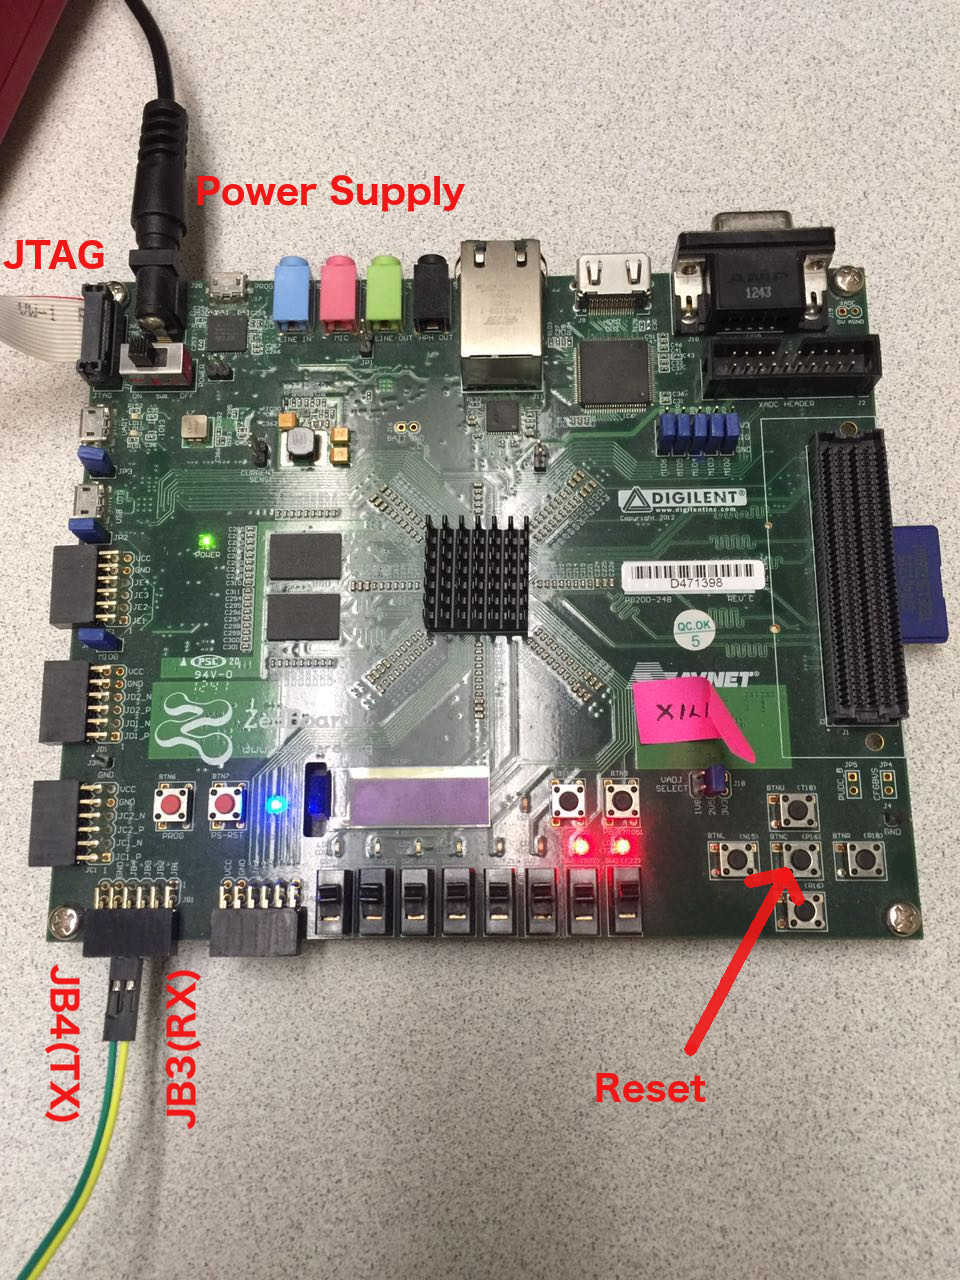
\includegraphics[width=8cm]{./fig/FPGA.jpg}
\centering
\end{figure}

\begin{figure}[h]
\caption{UART module connection setup}
\label{uart}
\includegraphics[width=8cm]{./fig/UART.jpg}
\centering
\end{figure}

\clearpage

% \subsubsection{Run on R2 FPGA}
% We fetched absolute position sensor (APS) data in the hardware. There are two APSs: APS1 and APS2. Each APS is stored in a 19bit raw data format. Figure.\ref{aps} show the relationship of raw APS data value and the real radius.\\
% In our design, we configured the at\_checker.vhd to sum up APS1 and APS2. In this way, the sum will keep around a constant value (e.g. x0\_0050). When we apply torque on the joint, the sum will shift based on the torque. The shift should within a reasonable range. In Figure.\ref{aps} (c), the red line is the sum with 0 torque applied. The green area is the reasonable shift range we defined. The task of the R2U2 is to measure whether the sum is in the green area or not.
% \begin{figure}[h]
% \caption{Signal Graph of APS1, APS2 and the Combination}
% \label{aps}
% 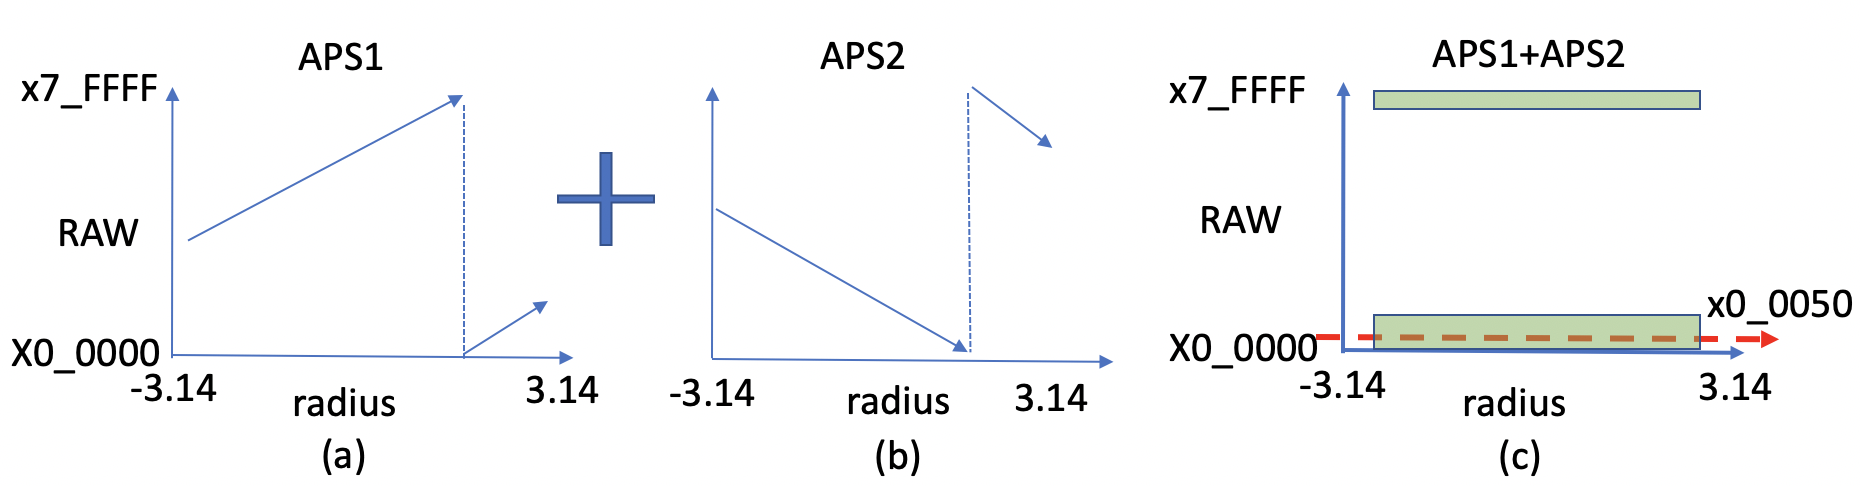
\includegraphics[width=16cm]{./fig/APS.png}
% \centering
% \end{figure}




% \subsection{Workflow}
% \begin{figure}[h]
% \caption{Demo Workflow}
% \label{workflow}
% 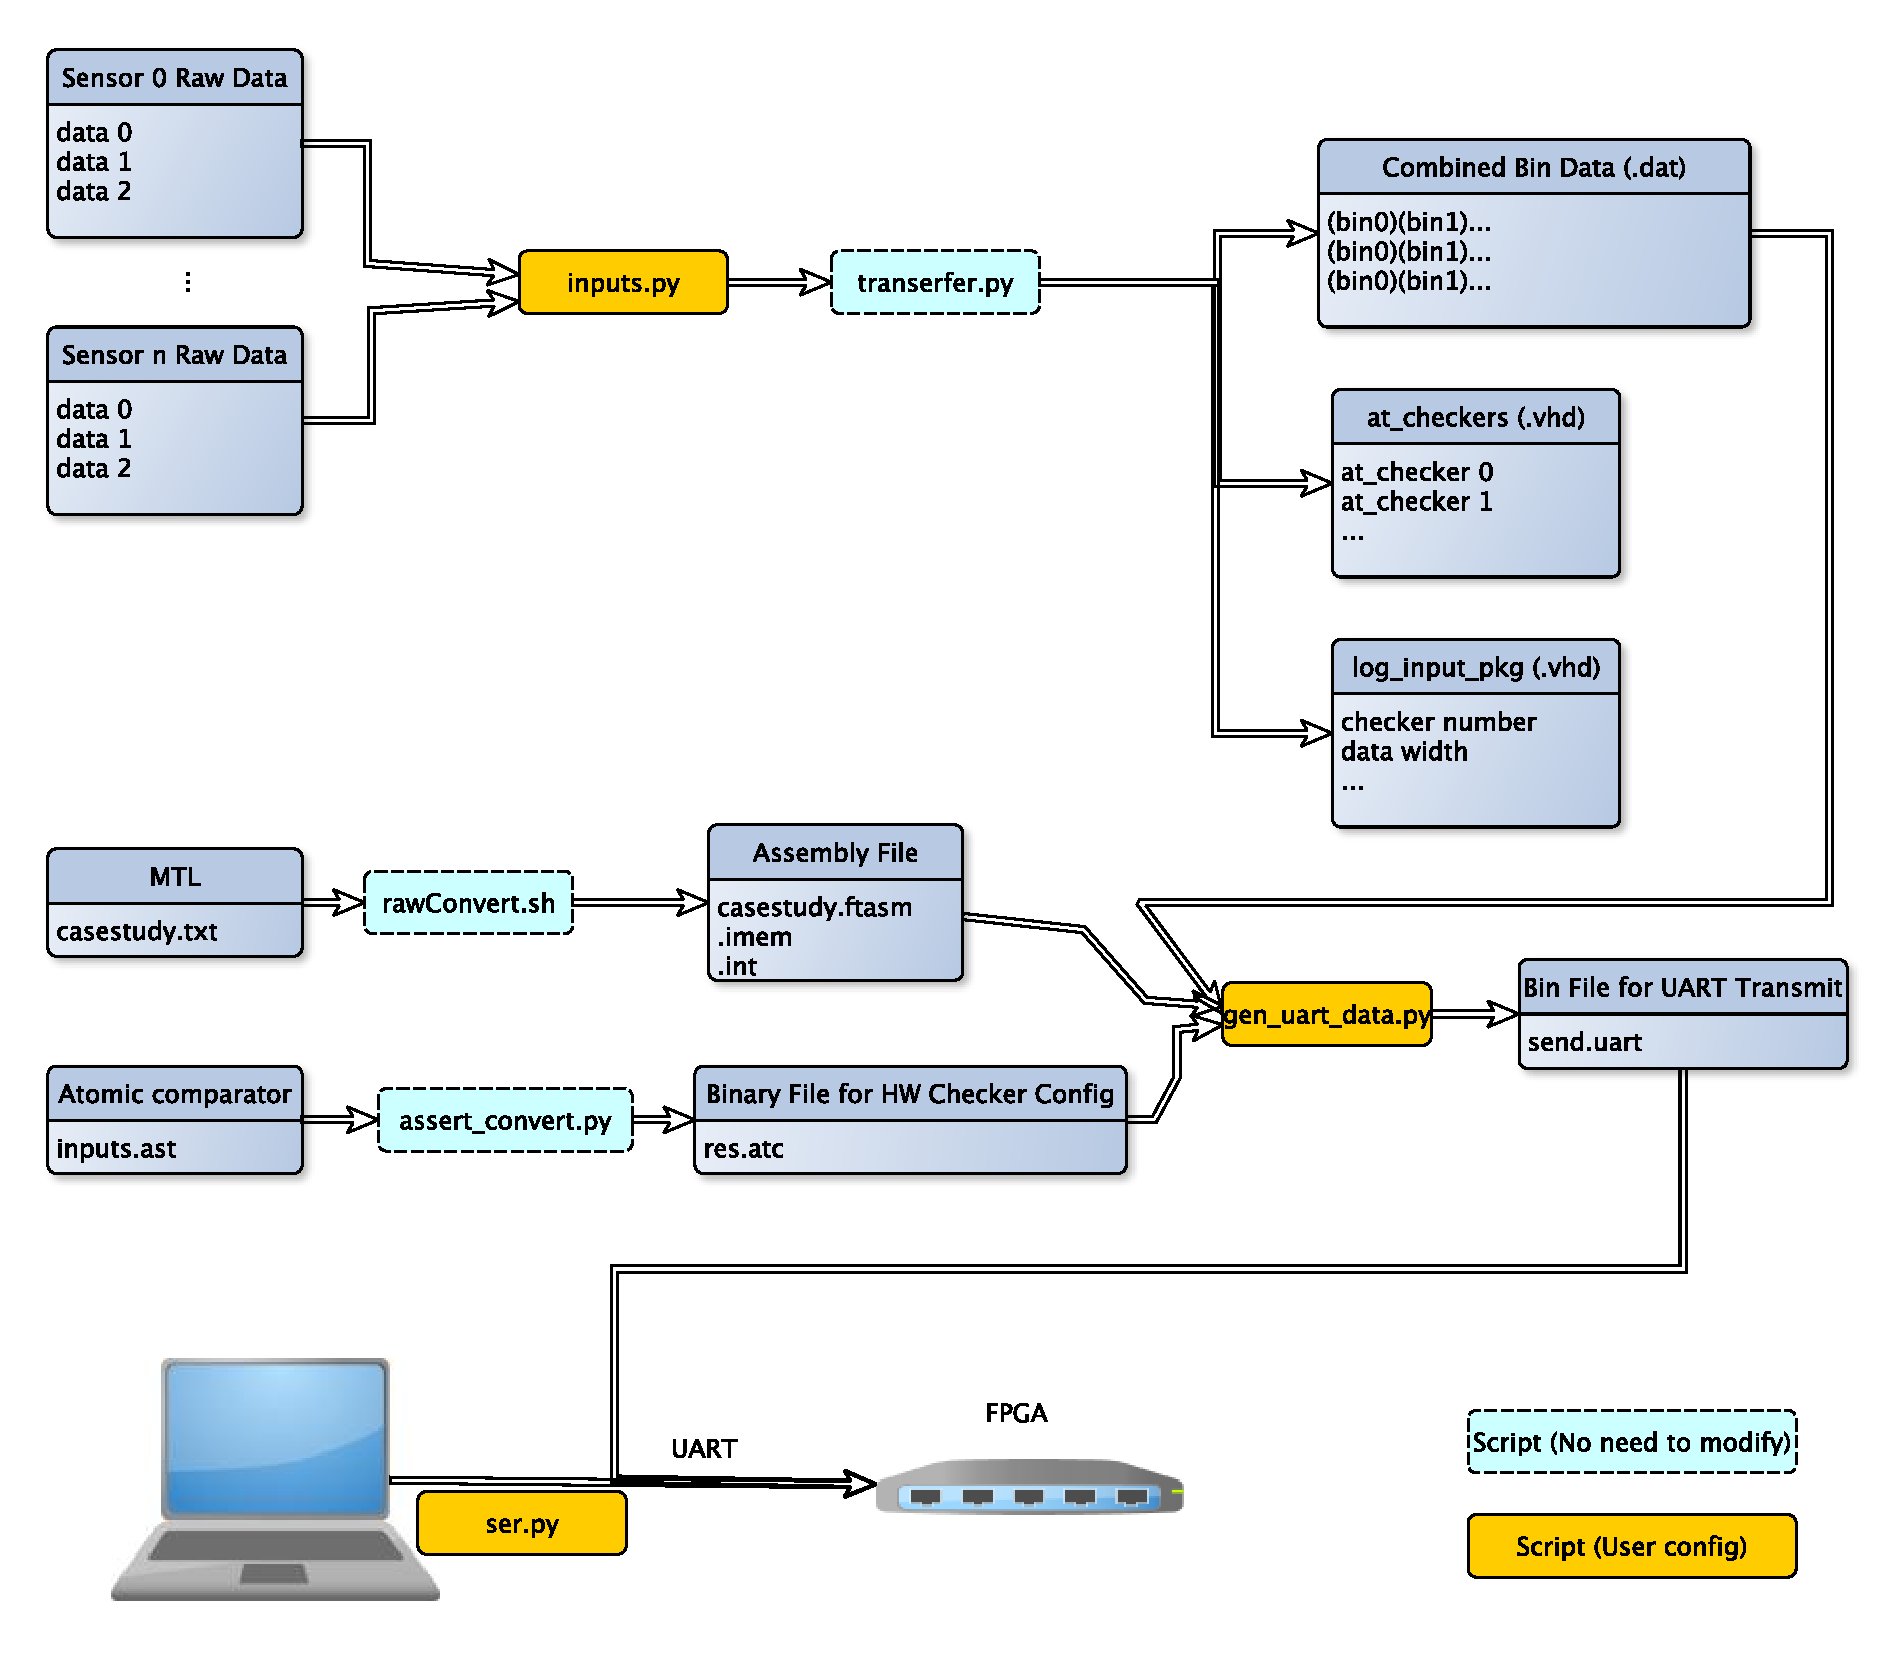
\includegraphics[width=15cm]{./fig/r2u2_process.eps}
% \centering
% \end{figure}

% \clearpage

% \subsection{Design Structure}
% \begin{figure}[h]
% \caption{Structure of R2U2 Hardware Component}
% \label{workflow}
% 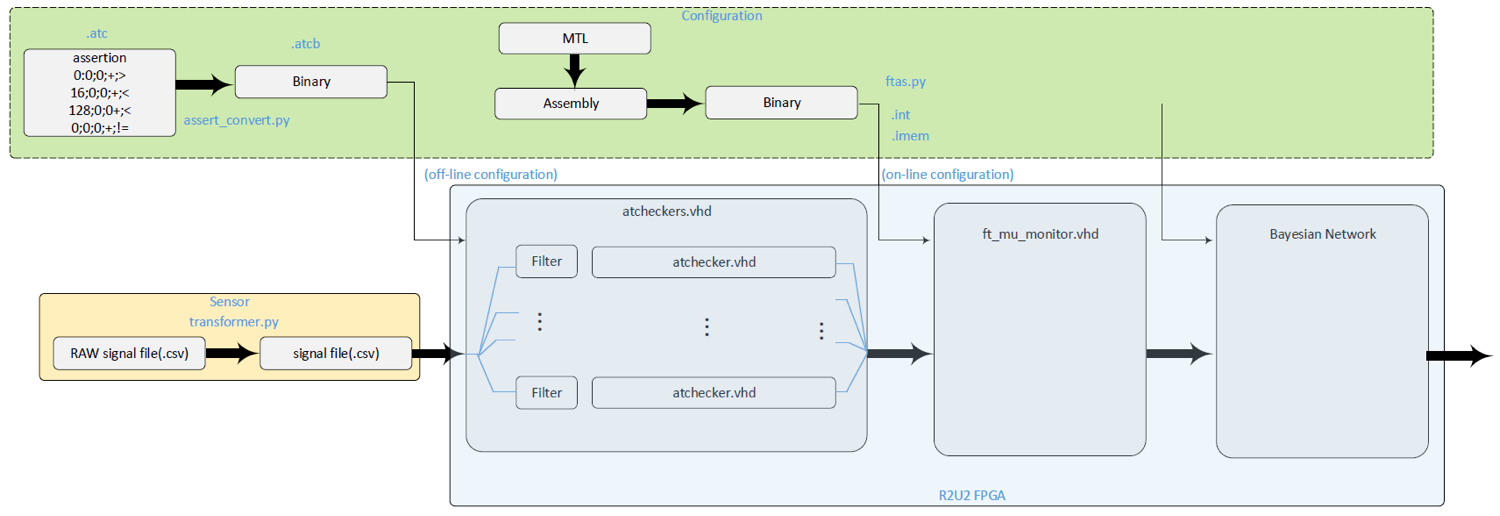
\includegraphics[width=16cm]{./fig/project_structure.png}
% \centering
% \end{figure}

\clearpage





\appendix
\section{\\File Structure}
\begin{forest}
  for tree={
    font=\ttfamily,
    grow'=0,
    child anchor=west,
    parent anchor=south,
    anchor=west,
    calign=first,
    inner xsep=7pt,
    edge path={
      \noexpand\path [draw, \forestoption{edge}]
      (!u.south west) +(7.5pt,0) |- (.child anchor) pic {folder} \forestoption{edge label};
    },
    before typesetting nodes={
      if n=1
        {insert before={[,phantom]}}
        {}
    },
    fit=band,
    before computing xy={l=15pt},
  }
[scripts/
  [config.py (setup all the configuration parameters in this file)
  ]
  [at\_checker/(generate VHDL file for atomic checker)
    [inputs.py(list all the atomic checkers and signals width here)
    ]
  ]
	[ftAssembler/
		[casestudy.txt (write the MTL formula here)
		]
		[rawConvert.sh (script to compile MTL into assemply)
		]
		[compiler/
		]
	]
  [sensor\_data.dat (write the sensor data here for simulation purpose)
  ]
	[gen\_log\_data.py (convert the sensor\_data.dat into binary format)
	]
	]
	[inputs.ast (configure each atomic checker)
	]
	[assert\_convert.py (convert inputs.ast into binary format)
	]
	[gen\_uart\_data.py (convert all the binary configuration file into Byte, which will send through UART)
	]
  [ser.py (python script to configure FPGA and read result through UART)
  ]
]
\end{forest}



\section{\\Details of Scripts and Files}
\subsection{inputs.py}\label{inputs.py}
(only compatiable with python 2.x)\\
Processing raw data file (similar to .csv) to the data format we want.\\
Parameters and functions:
\begin{enumerate}
	\item DATA\_SET: Raw data set file
	\item class subclass(CsvParser): \\
e.g.
\begin{lstlisting}[language=Python]
class Gs111m(CsvParser):
	def __init__(self):
		CsvParser.__init__(self)
		self.file = DATA_SET + "/gs111m_0.csv"
		self.addConfig(9, "float", 10, 24, "roll_angle", "in 1/2^10 rad")
		self.addConfig(8, "float", 10, 24, "pitch_angle", "in 1/2^10 rad")
\end{lstlisting}
Comment: Create a subclass. It will subtract the data you mentioned in \textbf{self.addConfig} and output the processed data into \textbf{self.file}
The self.file will look like:
\begin{center}
\begin{tabular}{ c|c}
 \hline
 roll\_angle & pitch\_angle \\
 \hline
 -42 & 12 \\
 \hline
 -34 & 6\\
 \hline
 -25 & 3\\
 ...&...
\end{tabular}
\end{center}
$\triangleright$ self.addConfig(channel, type, comma, width, name, comment)\\
@ channel: Column of the data in the raw data file.\\
@ type: Float or not. If it's float, write "float", else leave null.\\
@ comma: Only used for floating data type. It specifies how many fraction bit in binary you want to reserve during the conversion.\\
@ width: Number of bits for this data.\\
@ name: Specify the name of the column data. This will affect the name used in the .vhd code.\\
@ comment: Add any comment in string as you want.

\item class subclass(AtChecker):\\
e.g.
\begin{lstlisting}[language=Python]
class AtCheckerConfig(AtChecker):
	def __init__(self, inputFiles):
		AtChecker.__init__(self, inputFiles)
		self.add("pitch_angle", "", 1, "", "", "", "")
		self.add("roll_angle", "", 1, "", "", "", "")
\end{lstlisting}
Comment: Create a subclass. The subclass specifies the filters, number of atomic checkers, etc.. The class will affect at\_checker.vhd\\
$\triangleright$ self.add(input1, input2, count, filter1, filter2, rate1, rate2)\\
@ input1: First input to the at\_checker\\
@ input2: Second input to the at\_checker, usually used for compare with @input1. We can leave it as a null string "".\\
@ count: How many atomic checkers you want for this signal.\\
@ filter1: Hardware filter you want to use for input1. The filter name should be the same as the hardware filter component\\
@ filter2: Hardware filter you want to use for input2.\\
@ rate1: Signal delta during each sampling clk for input1. Leave null if you want to monitor signal delta.\\
@ rate2: Signal delta during each sampling clk for input2.

\end{enumerate}


\subsection{input.ast}\label{input.ast}
Atomic assertion file. Specify the at\_checker.vhd operation mode. For details, refer to \textbf{Performance\_Aware\_Hardware\_Runtime\_Monitors.pdf}.
\\
e.g.\\
\begin{tabular}{|p{0.98\textwidth}|}
\hline
-16;0;0;+;$>$\\
1;0;0;+;$=$\\
100;0;0;+;$>$\\
\hline
\end{tabular}
\\
\begin{figure}[h]
\caption{Atomic checker block}
\label{ac}
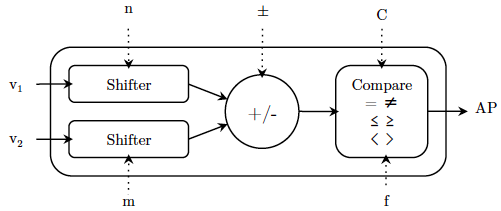
\includegraphics[width=8cm]{./fig/ast.png}
\centering
\end{figure}
Each line specifies the configuration for one atomic checker block. Consider the structure
of an atomic checker, depicted in Figure.\ref{ac}, then each line in the configuration file reads as:
C;n;m;+/-;f.

\subsection{gen\_uart\_data.py}\label{gendata.py}
Generate uart data byte by byte. Requires \textbf{.atc}, \textbf{.imem}, \textbf{.int} and \textbf{.dat} as input. I suggest leave the \textbf{.dat} file empty for the demo purpose.\\
%\begin{enumerate}
%	\item
%	\item class subclass(CsvParser): \\
%\end{enumerate}
Parameters:\\
@ SETUP\_DATA\_WIDTH\_extend\_byte: \textbf{.atc} file configuration data width.\\
@ SETUP\_ADDR\_WIDTH\_extend\_byte: \textbf{.atc} file configuration address width.\\
@ DATA\_BYTE\_WIDTH\_extend\_byte: binary logged data bit width (each line width of \textcolor{purple!30}{logged\_data.dat}).\\
These three parameters should be the same as in \textcolor{purple!30}{R2U2\_pkg.vhd}.

 \subsection{ser.py}\label{ser.py}

 \begin{enumerate}
 	\item serial.Serial()\\
	e.g.
	\begin{lstlisting}[language=Python]
ser = serial.Serial(
    port='/dev/ttyUSB0',
    timeout=0,
    # baudrate=9600,
    # parity=serial.PARITY_ODD,
    # stopbits=serial.STOPBITS_TWO,
    # bytesize=serial.SEVENBITS
 )
	\end{lstlisting}

Comment: By default, it is 9600 baud rate 8IN1 mode. You only need to specify the PC port that the UART is connecting to.
	\item parameters:
	@ DATA\_BYTE\_WIDTH\_extend\_byte: (same as \textcolor{purple!30}{gen\_uart\_data.py})
  \end{enumerate}

\end{document}
